\newpage
\section{Viewers}
\label{sec:viewers}

\begin{description}
 %------------------------------------------------------------------------------
\addcontentsline{toc}{subsection}{btkSlicesMotionViewer}
\item[btkSlicesMotionViewer]: Construct a VTK polydata wich outline the slice for each input. Transforms can be given in output the option \texttt{-r} will open a render window.
A typical use of this program is to visualize slice by slice transformation onto volume. See figure~\ref{fig:btkSlicesMotionViewer}.

Recommended usage: \texttt{btkSlicesMotionViewer -i ana01.nii.gz $\cdots$ -i anaN.nii.gz -t transform01.txt $\cdots$ -t transformN.txt -o PolyData01.vtk $\cdots$ -o PolyDataN.vtk -r }

Note that the only required arguments are the inputs and outputs.

\begin{figure}[t]
\centering
\begin{tabular}{ccc}
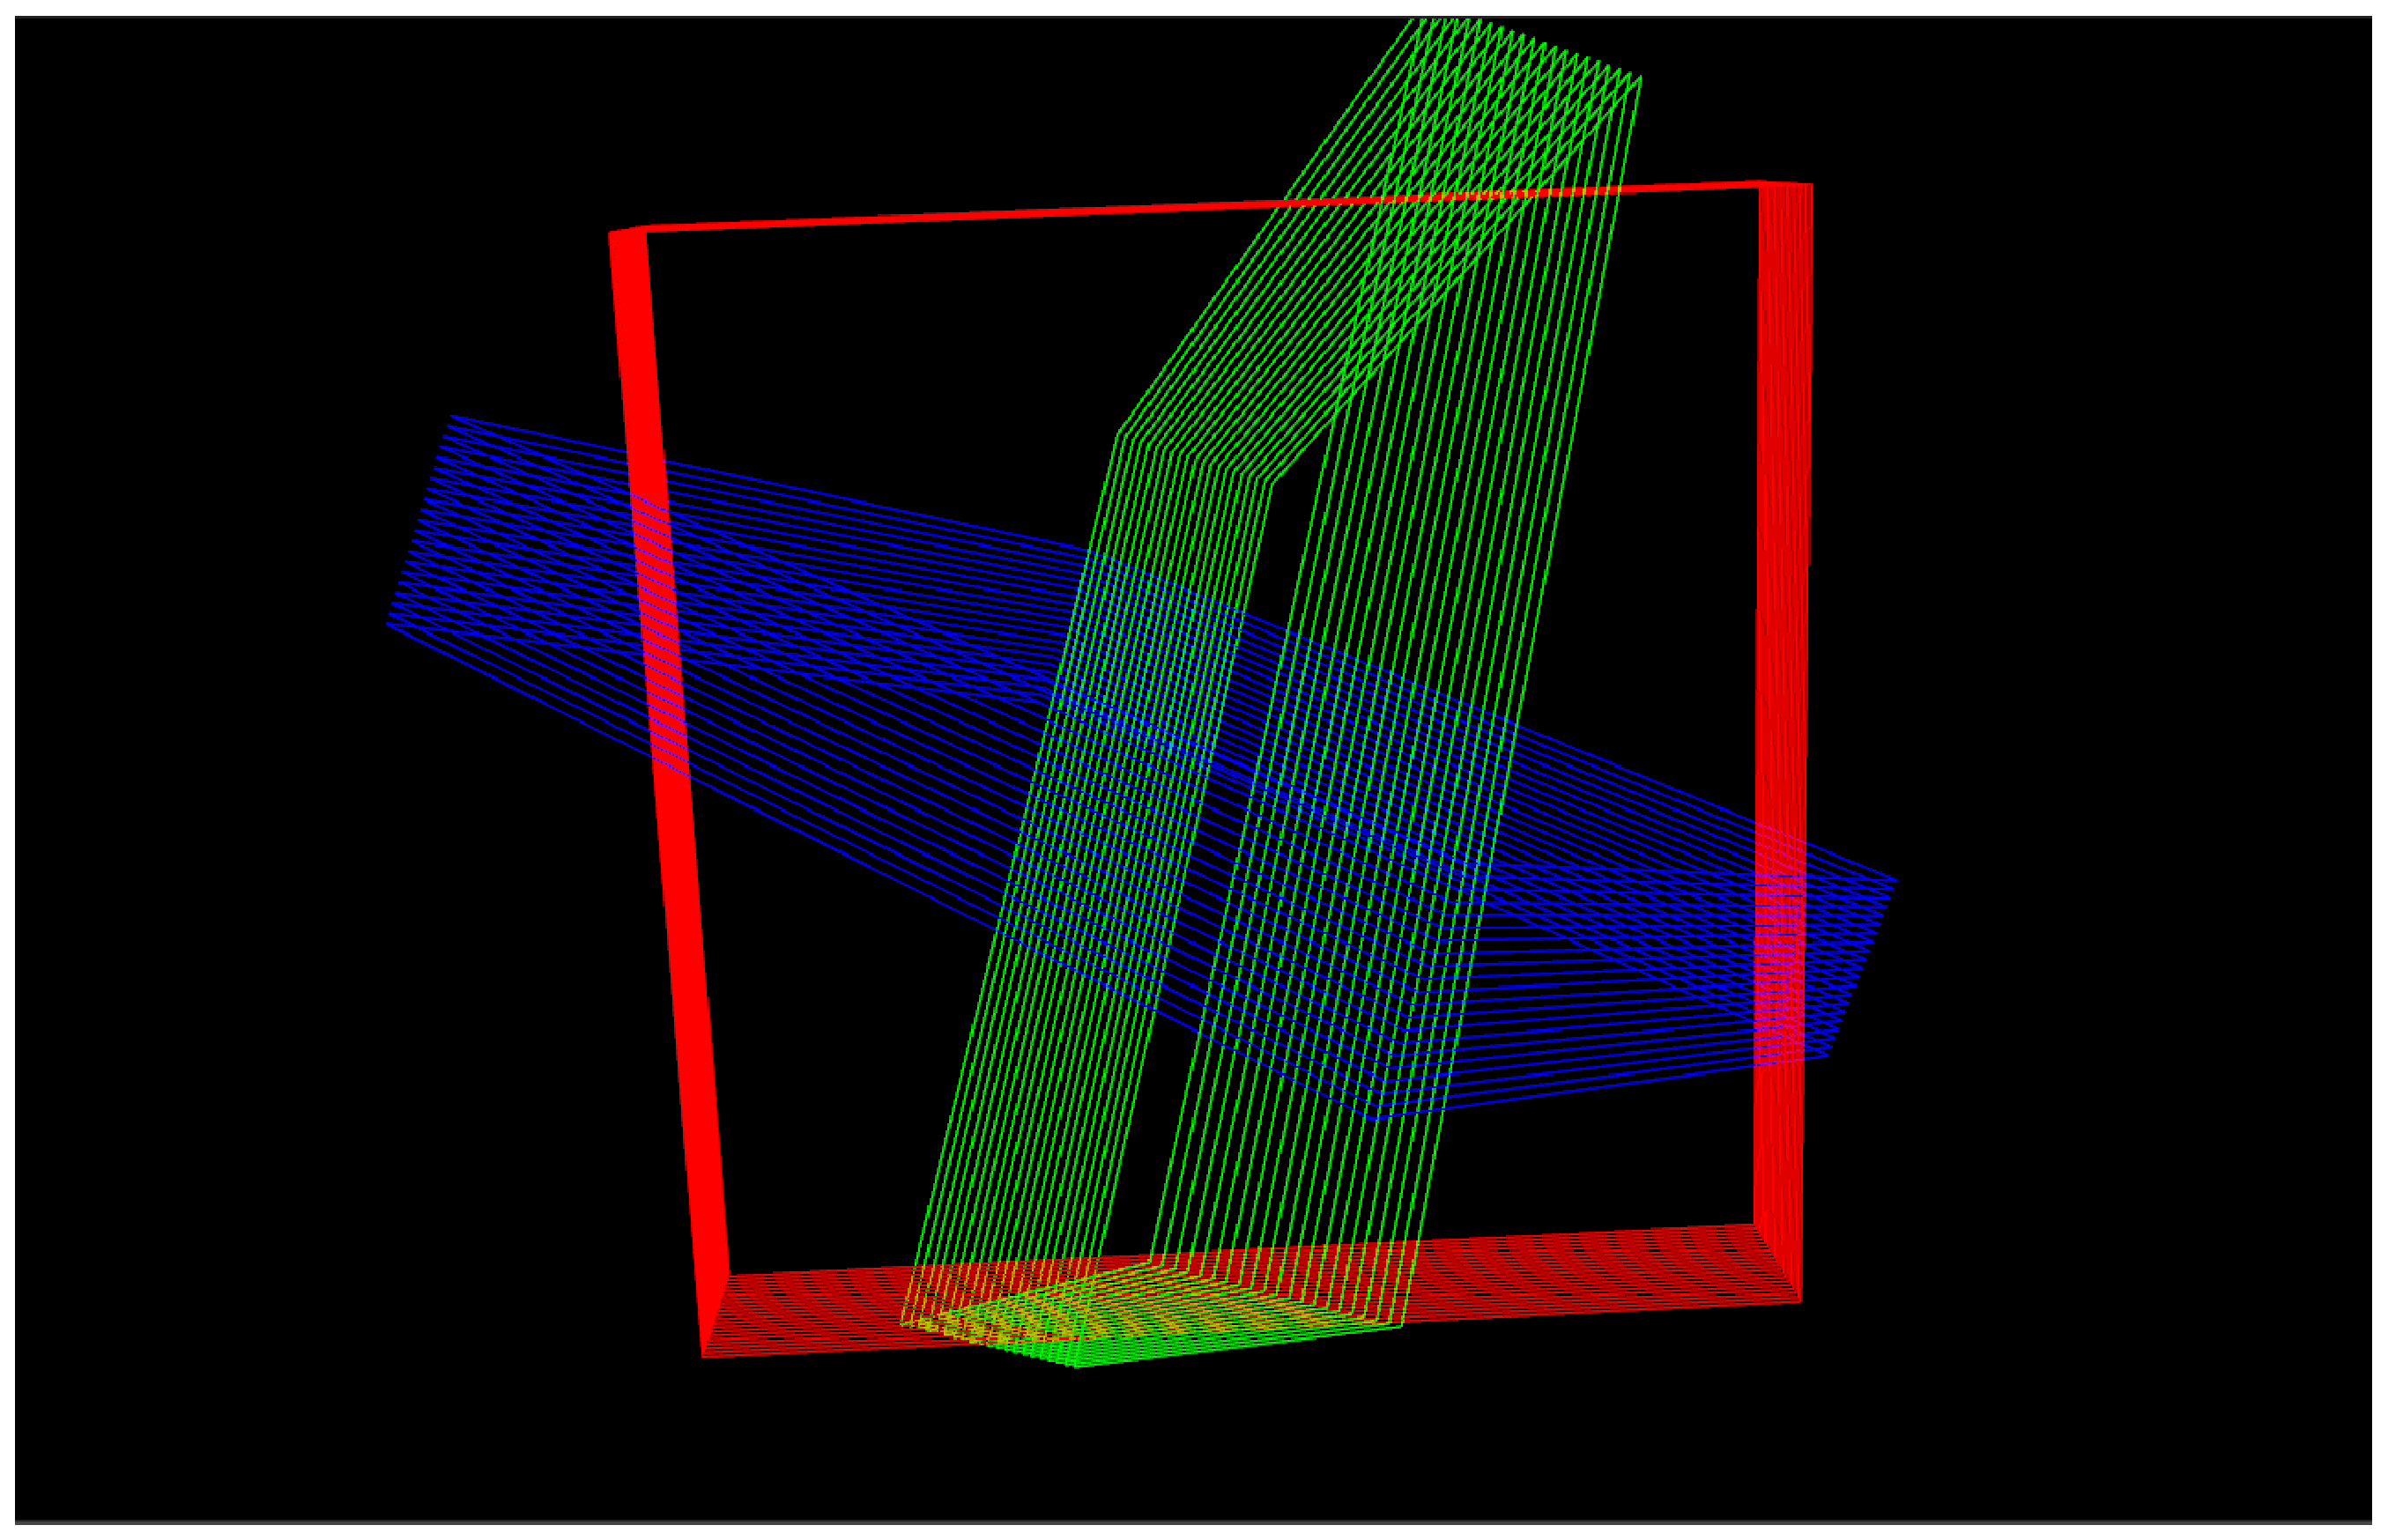
\includegraphics[width=0.5\columnwidth]{btkSlicesMotionViewer.eps}
\end{tabular}
\caption{Example of a render of three polydatas (axial, coronal, and sagital).
\texttt{btkSlicesMotionViewer}.}
\label{fig:btkSlicesMotionViewer}
\end{figure}

%------------------------------------------------------------------------------
\addcontentsline{toc}{subsection}{btkViewer}
\item[btkViewer]:
%------------------------------------------------------------------------------

\end{description}

